\documentclass[11pt]{article}
\usepackage[margin=2.2cm]{geometry}
\usepackage{amsmath,tikz}
\usetikzlibrary{arrows.meta,decorations.markings}
\title{Numerical evaluation of the $V\to q\bar q g$ finite remainders:\\ boundary values and transport}
\date{}
\begin{document}
\maketitle

\paragraph{Setup.}
Every finite remainder is a sum $\sum q\,R_r(y,z)\,T_g\,c_m$ of rational functions, constants and 579 pure functions
$T_g$. The $T_g$ are iterated integrals with base point $(x,y)=(0,0)$, where every non-empty integral vanishes after
shuffle regularisation. They satisfy a closed canonical system $dF=\sum_k d\log W_k\,M_k F$ of 503 functions, which
we integrate numerically.

\paragraph{Boundary values (computed once).}
The origin is singular, so we do not start there. We expand in series instead (see the figure):
\begin{enumerate}
\item along the edge $x=0$, from $(0,0)$ to $(0,\tfrac12)$, as a series in $y$. On the edge only $y=0,1$ are
  singular, and the regularisation sets $\log y\to0$ at the origin;
\item off the edge at fixed $y=\tfrac12$, as a series in $\sqrt{x}$ (the square-root letters go like $\sqrt x$), up to
  $S=(0.02,\tfrac12)$. Here $\log x\to0$ at $x=0$;
\item one numerical transport (Bulirsch--Stoer) from $S$ to the central point $P_0=(0.3,0.3)$.
\end{enumerate}
The values at $P_0$ are stored once and for all and shipped with the evaluator. The mirror construction, through
$(\tfrac12,0)$ and $(\tfrac12,0.02)$, gives an independent set, used only for the error estimate.

\begin{center}
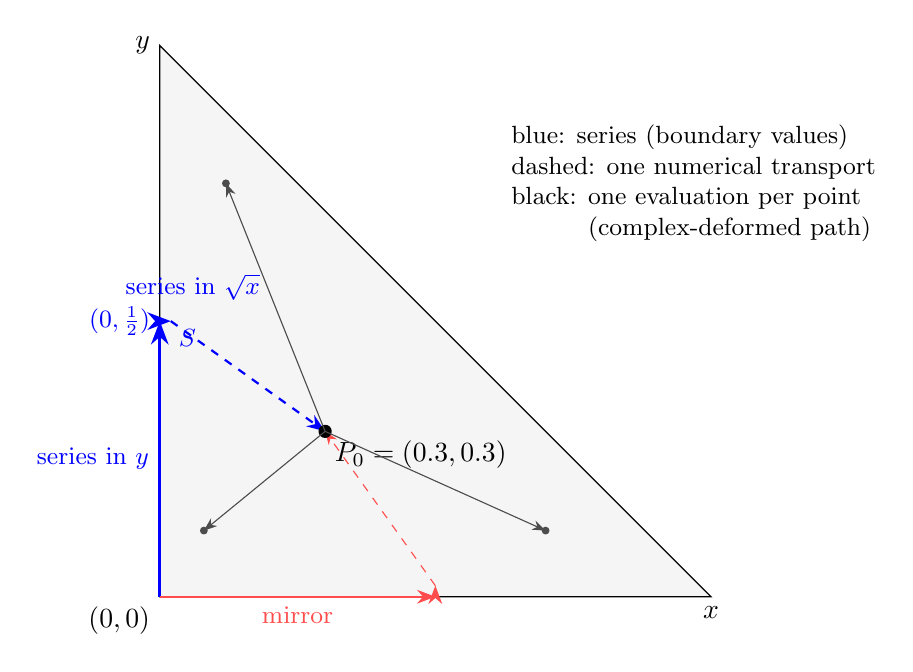
\begin{tikzpicture}[scale=7,>=Stealth]
  \fill[gray!8] (0,0)--(1,0)--(0,1)--cycle; \draw (0,0)--(1,0)--(0,1)--cycle;
  \node[below left] at (0,0) {$(0,0)$}; \node[below] at (1,0) {$x$}; \node[left] at (0,1) {$y$};
  % x-first construction
  \draw[very thick,blue,->] (0,0)--(0,0.5) node[midway,left] {\small series in $y$};
  \draw[very thick,blue,->] (0,0.5)--(0.02,0.5) node[below right=-1pt] {\small $S$};
  \node[blue,left] at (0,0.5) {\small $(0,\frac12)$};
  \draw[thick,blue,dashed,->] (0.02,0.5)--(0.3,0.3);
  % mirror
  \draw[thick,red!70,->] (0,0)--(0.5,0) node[midway,below] {\small mirror};
  \draw[thick,red!70,->] (0.5,0)--(0.5,0.02);
  \draw[red!70,dashed,->] (0.5,0.02)--(0.3,0.3);
  % hub and evaluations
  \fill (0.3,0.3) circle (0.012) node[below right] {$P_0=(0.3,0.3)$};
  \foreach \p in {(0.12,0.75),(0.7,0.12),(0.08,0.12)}
     \draw[->,black!70] (0.3,0.3) -- \p node[circle,fill,inner sep=1pt] {};
  \node[blue,font=\small,above] at (0.06,0.52) {series in $\sqrt{x}$};
  \node[align=left,font=\small,anchor=west] at (0.62,0.75) {blue: series (boundary values)\\ dashed: one numerical transport\\ black: one evaluation per point\\ \phantom{black: }(complex-deformed path)};
\end{tikzpicture}
\end{center}

\paragraph{Evaluation at a point $P$.}
We integrate the system from $P_0$ to $P$ along a straight path, deformed into the complex plane
($z(t)=P_0+(t+4i\delta\,t(1-t))(P-P_0)$). Three refinements:
\begin{itemize}
\item \emph{Spurious letters.} Six letters vanish on curves inside the triangle. The amplitude is smooth there, but
  the equations are not. The deformation $\delta$ is chosen so that the complex path stays away from their zeros.
\item \emph{Points on a spurious curve.} Such a point is replaced by the symmetric average of $P\pm h\,n$,
  $P\pm 2h\,n$, $P\pm 3h\,n$ across the curve ($n$ its normal), which is accurate to $O(h^6)$.
\item \emph{Error estimate.} Each point is evaluated a second time, from the mirror boundary values and on another
  path; the estimate is ten times the difference.
\end{itemize}
In the bulk the accuracy is about $10^{-12}$, and about $10^{-13}$ against the exact planar results. Near the edges
double precision loses digits, which the error estimate reports; there the corner expansions take over.

\end{document}
